\begin{figure}[h] 
\centering 
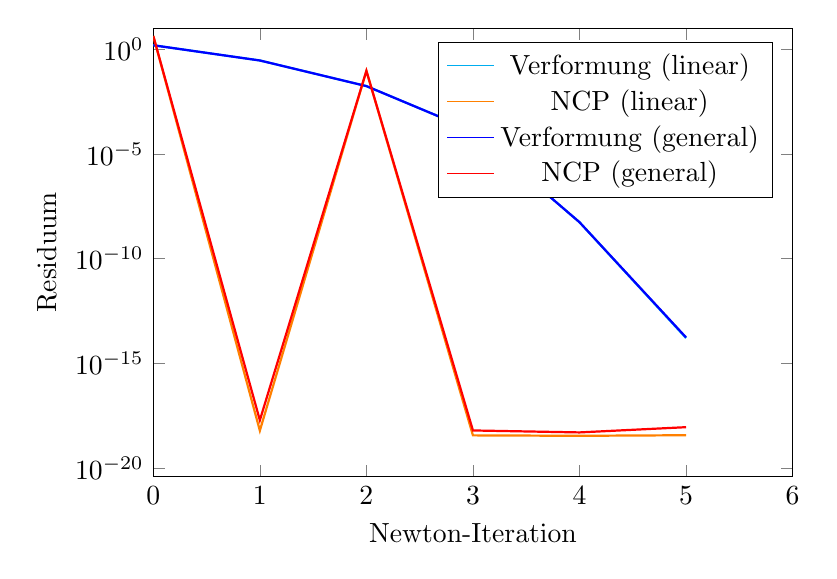
\begin{tikzpicture}[every plot/.append style={thick}] 
\begin{axis}[ 
label style={font=\normalsize}, 
xlabel={Newton-Iteration}, 
ylabel={Residuum}, 
xmin=0, xmax=6, 
ymode=log, 
ymin=0, ymax=10, 
width=0.8\textwidth, 
height=0.6\textwidth, 
legend pos=north east, 
legend style={cells={align=left}}, 
grid style=dashed, 
] 
\addplot[ 
color=cyan, 
] 
coordinates { 
(0, 1.54e+00)(1, 2.89e-01)(2, 1.73e-02)(3, 1.28e-04)(4, 5.53e-09)(5, 1.64e-14)}; 
\addlegendentry{Verformung (linear)} 
\addplot[ 
color=orange, 
] 
coordinates { 
(0, 4.26e+00)(1, 6.23e-19)(2, 9.23e-02)(3, 3.70e-19)(4, 3.53e-19)(5, 3.76e-19)}; 
\addlegendentry{NCP (linear)} 
\addplot[ 
color=blue, 
] 
coordinates { 
(0, 1.54e+00)(1, 2.89e-01)(2, 1.73e-02)(3, 1.28e-04)(4, 5.53e-09)(5, 1.76e-14)}; 
\addlegendentry{Verformung (general)} 
\addplot[ 
color=red, 
] 
coordinates { 
(0, 4.26e+00)(1, 1.96e-18)(2, 9.23e-02)(3, 6.35e-19)(4, 5.12e-19)(5, 9.11e-19)}; 
\addlegendentry{NCP (general)} 
\end{axis} 
\end{tikzpicture} 
\caption{Residuen des Stoffgesetzes 'Neo Hooke' mit Hinderniss 'Spitze' und 2178 Freiheitsgraden für die Verschiebung.} 
\label{fiq:NeoHooke_Spitze_level4} 
\end{figure} 
